\documentclass[titlepage]{article}
\usepackage[utf8]{inputenc}
\usepackage[margin=1in]{geometry}

\title{%
  Math 348: Cryptography - Final Paper \\
  \large Pseudorandom Number Generation, Theory and Practice
}
\author{Victor Zhang}
\date{May 7, 2021}

\usepackage{amsmath}
\usepackage{amsfonts}
\usepackage[square,numbers]{natbib}
\usepackage{url}
\usepackage{graphicx}
% \usepackage{changepage}
\usepackage{amssymb}
\usepackage{xfrac}
% \usepackage{bm}
% \usepackage{empheq}
\usepackage{amsthm}
\usepackage{dirtytalk}
\usepackage{cleveref}
\usepackage{setspace}
\usepackage{tikz}

\bibliographystyle{abbrvnat}
\theoremstyle{definition}
\newtheorem{definition}{Definition}[section]

\tikzset{every picture/.style={line width=0.75pt}} %set default line width to 0.75pt        

\newcommand{\contra}{\raisebox{\depth}{\#}}

\newenvironment{myindentpar}[1]
  {\begin{list}{}
          {\setlength{\leftmargin}{#1}
          \setlength{\rightmargin}{#1}}
          \item[]
  }
  {\end{list}}

\pagestyle{empty}
\doublespacing

\begin{document}

\maketitle
% \begin{center}
% {\huge Econ 482 \hspace{0.5cm} HW 3}\
% {\Large \textbf{Victor Zhang}}\
% {\Large February 18, 2020}
% \end{center}

\section{Introduction}
Computers are by nature deterministic machines. With a given starting state and list of instructions, the resulting state will be identical every single time. This reliability has made computers an indispensable part of the modern world. But this predictability also makes computers bad at producing truly random behavior. Since many applications make use of random numbers, this motivates the study of \textit{pseudo-random number generators}, deterministic algorithms to produce seemingly random output.

\section{Theory}
Before we can discuss pseudorandom generation, it's useful to define our criteria of randomness.
\subsection{Pseudorandom Functions}
Let $I_k$ be the set of all bitstrings of length $k$. Let $H_k$ be the set of all functions $f: I_k \to I_k$. Note that $|H_k| = 2^{k \cdot 2^k}$, a truly astronomical number for even small $k$. By a family of functions $F$ we mean a set $\{F_k\}$, where $F_k \subset H_k$ is a multiset of functions $I_k \to I_k$.

\begin{definition}[Goldreich, Goldwasser, and Micali \cite{GGS}]
A \textit{polytime statistical test for functions} is a probabilistic polytime algorithm $A$ that, given input $k$ and access to an oracle machine $O_f$ for a function $f: I_k \to I_k$, guesses whether the function is truly random. A family $F$ \textit{passes the test A} if for any polynomial function $Q$ and sufficiently large $k$
$$|p_k^F - p_k^H| < \frac{1}{Q(k)}$$
where $p_k^H$ is the probability $A$ guesses a truly random function (sampled uniformly from $H_k$) is random, and $p_k^F$ is the probability $A$ guesses a function $f \in F$ is truly random.
\end{definition}

Informally, a function $f$ is \say{judged} by $A$, which makes polynomially many calls to $f$ before making a decision. If $F$ is sufficiently \say{random-looking}, $O_f$ will give essentially no information about whether $f \in F$ or $f$ is truly random.

We will consider the combination of a function $f \in F$ and truly random seed $k$ to be adequately random if $F$ passes all polytime statistical tests. Readers familiar with the theory of hash functions will notice similarities between the definition of random functions and random hash functions. In fact, we will show a pseudorandom generation technique in section 4 that exploits the nice statistical guarantees of sufficiently random hash functions.

Now that we have established formally the definition of random function families, we will give an equivalent intuitive definition that is easier to work with. Consider a \textit{psuedorandom number generator} (PRNG) to be an algorithm that takes as input an initial \textit{seed} value $k$ whose repeated execution mimics an adequately random function combination $(f,k)$. Without loss of generality, we also give the following definition which will be useful in the next section:

\begin{definition}\label{def:PRNG}
A \textit{pseudorandom number generator} or \textit{deterministic random bit generator} is a deterministic program $A$ that is initialized with a \textit{seed} value $k$ and whose execution produces bits such that the sequence of bits generated from repeated executions of $A$ is indistinguishable from a truly random bitstring. \cite{PractCrypt}
\end{definition}

It is important to note that since this PRNG has no sources of randomness except the seed, it is completely deterministic once initialized. In other words, if you take two copies of a PRNG and initialize them with the same seed, they will output identical bitstrings. Thus, engineers must be careful to choose a seed that is secret or otherwise truly random, lest their PRNGs be predictable and vulnerable to exploits \cite{NIST}.

\subsection{Cryptographically Secure Pseudorandom Generators}
For most intents and purposes, a PRNG that satisfies Definition~\ref{def:PRNG} is enough. But for cryptographic applications, we need our PRNGs to stand up to even the toughest adversarial attacks.

\begin{definition}\label{def:CSPRNG}
A \textit{cryptograpically secure pseudorandom generator} (CSPRNG) is a PRNG $P$ with the added conditions:
\begin{itemize}
\item Satisfies the \textbf{next-bit test}: Given the history of $n$ bits generated by $P$, there is no polytime algorithm to determine the $n+1$-th bit with more than random accuracy.
\item Withstands \textbf{state compomise attacks}: If an adversary knows the internal state of $P$, it is infeasible to reproduce the bits generated prior to the compromising attack. \cite{PractCrypt}
\end{itemize}
\end{definition}

Essentially, an adversary cannot use information about a CSPRNG to gain any new information about its operation. We cannot predict the future without knowing the seed, even with full knowledge of the past. If we know the seed, we can obviously determine the future, but we cannot \say{reverse-engineer} the seed to look back in time. These added guarantees are required to ward off all potential adversarial attacks. Even if the adversary wrote the program themselves, they would not be able to crack a CSPRNG.

\section{Basic PRNGs}
We begin our exploration of practical RNGs by discussing widely used examples of PRNGs. None of these are cryptographically secure PRNGs, which we discuss in section 4.

\subsection{Linear Congruential Generators}
Perhaps one of the most widely used and widely known pseudorandom generation techniques, linear congruential generators were first invented in the 50s as a quick and easy way of getting random bits \cite{LCG}.

\begin{definition}
A \textit{Linear Congruential Generator} (LCG) is an algorithm that generates a sequence of numbers $X_i$ based on the recurrence relation
$$X_{i+1} = (aX_i + c) \mod m$$
The seed $X_0$ is given as the initial condition.
\end{definition}
LCGs are characterized by having a long and predictable period after which the output loops. If we take $m$ to be a large prime and $c = 0$, the operation of RNG is identical to repeated multiplication in $\mathbb{F}_m$ and well-studied. If we choose $X_0 \in \mathbb{F}_m^\times$ the period is exactly $m-1$ and every element of $\mathbb{F}_m^\times$ will appear once \cite{Textbook}. However, unless $m$ is close to a power of 2, computing remainders mod $m$ is slow (compared to multiplication and addition).

If we choose $m$ to be a power of 2, we can perform mod operations by simple bit truncation, which is fast. For this reason, many LCG implementations choose $m$ to be a power of 2. If $c$ is correctly chosen, the period of this LCG can be equal to $m$ \cite{LCG,RNGs}. Even still, power-of-2 choices of $m$ suffer from a serious drawback. While the period of $X_i$ is long, the period of the bit truncations $X_i$\verb|%|$2^k$ is much shorter for $k < m$. Note that the lower $k$ bits of such an LCG also forms an LCG with modulus $2^k$ and thus have maximal period $2^k$. For instance, the last bit is constant, the last 2 bits have period 2, and the last 3 bits have period 4. Thus, most practical applications are careful to only take the higher-order bits only as the random output, since they have longer periods \cite{RNGs}.

In general, an LCG-based PRNG must choose its parameters carefully to avoid number-theoretic traps that cause execution to violate the randomness condition. This subtlety is often lost on developers, and there is a history of well-respected software libraries using terrible LCGs as their source of randomness. One of the most infamous examples is IBM's RANDU generator. It used the recurrence relation
$$V_{j+1} = 65539 V_{j} \!\!\!\mod 2^{31}$$
and returned random output as the floating point number
$$X_j = \frac{V_j}{2^{31}}$$
Developed in the 60s, this ill-conceived generator was certainly very fast to compute, but failed spectacularly on many statistical tests. For instance, when the results $(X_i, X_{i+1}, X_{i+2})$ are plotted as 3-dimensional points in space, the results of RANDU form 15 distinct 2-dimensional planes. This renders RANDU unsuitable for applications like Montecarlo simulations, which require multiple consecutive random numbers. The bad performance of RANDU was not noticed for many decades and as such was standard in many old libraries and compilers, calling into question the veracity of experiments during the 60s to 70s that used this as a source of randomness \cite{Knuth}.

\subsection{Mersenne Twister}
Proposed by Matsumoto and Nishimura in 1997, the Mersenne Twister is one of the most widely used PRNGs today. Developed specifically to correct the problems found in older PRNGs, its name comes from the fact that the period length is taken to be a Mersenne prime \cite{MT}.

The Mersenne Twister is an improvement on a class of generators known as \textit{generalized feedback shift registers} (GFSRs). To understand the Mersenne Twister, we need to first understand GFSRs.

\begin{definition}
A \textit{generalized feedback shift register} PRNG is a PRNG that generates output $X_{i+1}$ by applying a linear operator $T$ to the previous output $X_{i}$ \cite{GFSR}.
\end{definition}

For most intents and purposes, we may consider output $X_i$ to be bit vectors of length $n$ and $T$ to be an $n \times n$ bitmatrix. GFSRs has several advantages over LCGs, including an arbitrarily long period independent of any hardware limitations and much more random pseudorandom generation.

\begin{figure}
\centering
\begin{tikzpicture}[x=0.75pt,y=0.75pt,yscale=-1,xscale=1]
%uncomment if require: \path (0,317); %set diagram left start at 0, and has height of 317

%Straight Lines [id:da5048889088343349] 
\draw    (71,60) -- (71,108) ;
\draw [shift={(71,110)}, rotate = 270] [color={rgb, 255:red, 0; green, 0; blue, 0 }  ][line width=0.75]    (10.93,-3.29) .. controls (6.95,-1.4) and (3.31,-0.3) .. (0,0) .. controls (3.31,0.3) and (6.95,1.4) .. (10.93,3.29)   ;
%Shape: Rectangle [id:dp22067176451334336] 
\draw   (61,220) -- (61,120) -- (81,120) -- (81,220) -- cycle ;
%Straight Lines [id:da07872210030974114] 
\draw    (61,200) -- (81,200) ;
%Straight Lines [id:da6259769249227003] 
\draw    (61,180) -- (81,180) ;
%Straight Lines [id:da4329084260371985] 
\draw    (61,160) -- (81,160) ;
%Straight Lines [id:da8729037078792099] 
\draw    (61,140) -- (81,140) ;
%Shape: Rectangle [id:dp24317333321705448] 
\draw   (211,223) -- (211,123) -- (231,123) -- (231,223) -- cycle ;
%Straight Lines [id:da9592428599768572] 
\draw    (211,203) -- (231,203) ;
%Straight Lines [id:da8422413004103559] 
\draw    (211,183) -- (231,183) ;
%Straight Lines [id:da7923235785428235] 
\draw    (211,163) -- (231,163) ;
%Straight Lines [id:da4786820894850172] 
\draw    (211,143) -- (231,143) ;
%Straight Lines [id:da41618148103984276] 
\draw    (245,133) -- (283,133) ;
\draw [shift={(285,133)}, rotate = 180] [color={rgb, 255:red, 0; green, 0; blue, 0 }  ][line width=0.75]    (10.93,-3.29) .. controls (6.95,-1.4) and (3.31,-0.3) .. (0,0) .. controls (3.31,0.3) and (6.95,1.4) .. (10.93,3.29)   ;
%Straight Lines [id:da006296387212042065] 
\draw    (245,153) -- (283,153) ;
\draw [shift={(285,153)}, rotate = 180] [color={rgb, 255:red, 0; green, 0; blue, 0 }  ][line width=0.75]    (10.93,-3.29) .. controls (6.95,-1.4) and (3.31,-0.3) .. (0,0) .. controls (3.31,0.3) and (6.95,1.4) .. (10.93,3.29)   ;
%Straight Lines [id:da005748088034359] 
\draw    (245,173) -- (283,173) ;
\draw [shift={(285,173)}, rotate = 180] [color={rgb, 255:red, 0; green, 0; blue, 0 }  ][line width=0.75]    (10.93,-3.29) .. controls (6.95,-1.4) and (3.31,-0.3) .. (0,0) .. controls (3.31,0.3) and (6.95,1.4) .. (10.93,3.29)   ;
%Straight Lines [id:da5496780608479359] 
\draw    (245,213) -- (283,213) ;
\draw [shift={(285,213)}, rotate = 180] [color={rgb, 255:red, 0; green, 0; blue, 0 }  ][line width=0.75]    (10.93,-3.29) .. controls (6.95,-1.4) and (3.31,-0.3) .. (0,0) .. controls (3.31,0.3) and (6.95,1.4) .. (10.93,3.29)   ;
%Shape: Rectangle [id:dp0810464411552978] 
\draw   (411,223) -- (411,123) -- (431,123) -- (431,223) -- cycle ;
%Straight Lines [id:da6784685674534798] 
\draw    (411,203) -- (431,203) ;
%Straight Lines [id:da6753467423490247] 
\draw    (411,183) -- (431,183) ;
%Straight Lines [id:da03215492209862014] 
\draw    (411,163) -- (431,163) ;
%Straight Lines [id:da2900925793712441] 
\draw    (411,143) -- (431,143) ;
%Straight Lines [id:da303278453581292] 
\draw    (445,133) -- (483,133) ;
\draw [shift={(485,133)}, rotate = 180] [color={rgb, 255:red, 0; green, 0; blue, 0 }  ][line width=0.75]    (10.93,-3.29) .. controls (6.95,-1.4) and (3.31,-0.3) .. (0,0) .. controls (3.31,0.3) and (6.95,1.4) .. (10.93,3.29)   ;
%Straight Lines [id:da07482970728619898] 
\draw    (445,153) -- (483,153) ;
\draw [shift={(485,153)}, rotate = 180] [color={rgb, 255:red, 0; green, 0; blue, 0 }  ][line width=0.75]    (10.93,-3.29) .. controls (6.95,-1.4) and (3.31,-0.3) .. (0,0) .. controls (3.31,0.3) and (6.95,1.4) .. (10.93,3.29)   ;
%Straight Lines [id:da8501734170995012] 
\draw    (445,173) -- (483,173) ;
\draw [shift={(485,173)}, rotate = 180] [color={rgb, 255:red, 0; green, 0; blue, 0 }  ][line width=0.75]    (10.93,-3.29) .. controls (6.95,-1.4) and (3.31,-0.3) .. (0,0) .. controls (3.31,0.3) and (6.95,1.4) .. (10.93,3.29)   ;
%Straight Lines [id:da3296514297409303] 
\draw    (445,213) -- (483,213) ;
\draw [shift={(485,213)}, rotate = 180] [color={rgb, 255:red, 0; green, 0; blue, 0 }  ][line width=0.75]    (10.93,-3.29) .. controls (6.95,-1.4) and (3.31,-0.3) .. (0,0) .. controls (3.31,0.3) and (6.95,1.4) .. (10.93,3.29)   ;
%Curve Lines [id:da7007057243627508] 
\draw    (230,240) .. controls (354.87,378.31) and (358.47,40.41) .. (418.1,108.94) ;
\draw [shift={(419,110)}, rotate = 230.35] [color={rgb, 255:red, 0; green, 0; blue, 0 }  ][line width=0.75]    (10.93,-3.29) .. controls (6.95,-1.4) and (3.31,-0.3) .. (0,0) .. controls (3.31,0.3) and (6.95,1.4) .. (10.93,3.29)   ;
%Curve Lines [id:da6658946412138489] 
\draw    (61,240.35) .. controls (147.07,380.3) and (159.38,40.43) .. (219.1,108.94) ;
\draw [shift={(220,110)}, rotate = 230.35] [color={rgb, 255:red, 0; green, 0; blue, 0 }  ][line width=0.75]    (10.93,-3.29) .. controls (6.95,-1.4) and (3.31,-0.3) .. (0,0) .. controls (3.31,0.3) and (6.95,1.4) .. (10.93,3.29)   ;
%Curve Lines [id:da6251122353171024] 
\draw    (420,236.41) .. controls (544.87,374.71) and (548.47,36.81) .. (608.1,105.34) ;
\draw [shift={(609,106.41)}, rotate = 230.35] [color={rgb, 255:red, 0; green, 0; blue, 0 }  ][line width=0.75]    (10.93,-3.29) .. controls (6.95,-1.4) and (3.31,-0.3) .. (0,0) .. controls (3.31,0.3) and (6.95,1.4) .. (10.93,3.29)   ;

% Text Node
\draw (56,29) node [anchor=north west][inner sep=0.75pt]   [align=left] {{\fontfamily{pcr}\selectfont seed}};
% Text Node
\draw (36,162) node [anchor=north west][inner sep=0.75pt]   [align=left] {$\displaystyle A$};
% Text Node
\draw (86,72) node [anchor=north west][inner sep=0.75pt]   [align=left] {{\fontfamily{pcr}\selectfont init}};
% Text Node
\draw (177,165) node [anchor=north west][inner sep=0.75pt]   [align=left] {$\displaystyle VA$};
% Text Node
\draw (296,122) node [anchor=north west][inner sep=0.75pt]   [align=left] {$\displaystyle X_{1}$};
% Text Node
\draw (296,142) node [anchor=north west][inner sep=0.75pt]   [align=left] {$\displaystyle X_{2}$};
% Text Node
\draw (296,162) node [anchor=north west][inner sep=0.75pt]   [align=left] {$\displaystyle X_{3}$};
% Text Node
\draw (296,202) node [anchor=north west][inner sep=0.75pt]   [align=left] {$\displaystyle X_{n}$};
% Text Node
\draw (213,190) node [anchor=north west][inner sep=0.75pt]   [align=left] {...};
% Text Node
\draw (369,165) node [anchor=north west][inner sep=0.75pt]   [align=left] {$\displaystyle V^{2} A$};
% Text Node
\draw (496,122) node [anchor=north west][inner sep=0.75pt]   [align=left] {$\displaystyle X_{1}$};
% Text Node
\draw (496,142) node [anchor=north west][inner sep=0.75pt]   [align=left] {$\displaystyle X_{2}$};
% Text Node
\draw (496,162) node [anchor=north west][inner sep=0.75pt]   [align=left] {$\displaystyle X_{3}$};
% Text Node
\draw (496,202) node [anchor=north west][inner sep=0.75pt]   [align=left] {$\displaystyle X_{n}$};
% Text Node
\draw (413,190) node [anchor=north west][inner sep=0.75pt]   [align=left] {...};
% Text Node
\draw (327,249) node [anchor=north west][inner sep=0.75pt]   [align=left] {{\fontfamily{pcr}\selectfont twist}};
% Text Node
\draw (131,252) node [anchor=north west][inner sep=0.75pt]   [align=left] {{\fontfamily{pcr}\selectfont twist}};
% Text Node
\draw (517,245.41) node [anchor=north west][inner sep=0.75pt]   [align=left] {{\fontfamily{pcr}\selectfont twist}};
% Text Node
\draw (608,139) node [anchor=north west][inner sep=0.75pt]   [align=left] {.\\.\\.};

\end{tikzpicture}
\caption{Mersenne Twister Generation}
\label{fig:MT}
\end{figure}

The Mersenne Twister adds another level of complexity to a basic GSFR by \say{twisting} the operator $T$ at set intervals. In particular, it generates a list $A = \{a_1, \dots, a_n\}$ by applying a transformation $T$ to a seed value $a_1$. The $i$-th time a number is requested, it returns $Ta_i$ and updates $a_i$ to be this value. Every $n$ generations, it applies another transformation $V$ to each element in the list. This is shown in Figure~\ref{fig:MT}. The particulars of each transformation are not instructive to our discussion and thus omitted \cite{MT}.

The Mersenne Twister is usually implemented with period $2^{19937}-1$ and $n = 624$. This standard implementation is given the moniker MT19937 and is the default PRNG for many modern libraries \cite{MTWiki}. In contrast to RANDU, it stands up well to many modern statistical tests, but still fails for tests that detect linear generators, which the Mersenne Twister is. Despite this, it is a passable all-purpose PRNG and should be acceptable for most non-cryptographic applications \cite{MTWiki}.

\section{Cryptographically Secure PRNGs}
In this section we will discuss some PRNGs commonly used in cryptography. Specific example of uses in cryptography will be discussed in section 6.

\subsection{Block Ciphers in Counter Mode}
\begin{definition}
A \textit{block cipher} is a symmetric cipher that takes as input a block of plaintext bits $m$ and an encryption key $k$ of the same length and applies a reversible transformation $f$. That is,
$$f(m,k) = c, \;\; f(c,k) = m$$ \cite{Textbook}
\end{definition}
Secure block ciphers are commonly used to encrypt long messages sent over the Internet. For our purposes, they have some convenient properties. One of these is the so-called \textit{indistinguishable} property, that is, encrypted ciphertext is indistinguishable from random noise \cite{NIST}. This is very similar to Definition~\ref{def:PRNG}, which posits that the bitstring produced by a PRNG is indistinguishable from that produced by a random function. In fact, this is one of the motivating reasons to consider block ciphers as PRNGs. The other useful property is resistance to known ciphertext attacks. That is, the transformation $f$ does not preserve locality of input: Similar inputs will be transformed totally independently \cite{NIST}. These two properties justify the following PRNG:

\begin{definition}[A naive block cipher PRNG]
Choose secure block cipher $f$ and seed $k$. Maintain a counter $X_i$, initialized to 0. When a random number is requested, calculate and return $f(k,X_i)$. Increment $X_{i+1} = (X_i + 1) \!\!\!\mod m$, where $m$ is some large modulus.
\end{definition}

Due to the two properties of secure block ciphers, this is clearly a PRNG. Because of the indistinguishable property, it also satisfies the next-bit test. However, it fails to proect against state-compromise attacks. Since a block cipher is symmetric, knowing the key and the counter is enough to recreate the entire prior sequence.

We may naively try to protect against state-compromise attacks by obfuscating the counter $X_{i}$, perhaps by using a Mersenne Twister or other PRNG to successively calculate values of $X_i$. But since none of the PRNGs discussed so far are cryptographically secure, the resulting obfuscation can be undone through the same state-compromising attack and we are left with the same problem. A logical next step is to try obfuscation with a method that isn't so easily cracked. This gives us the following (provably cryptographically-secure) PRNG:

\begin{definition}[Petit et al. 2008 \cite{Petit}]
Choose secure block cipher instances $E, E^*$, public initial value $IV = x_0$, and seeds $k_0, k_0^*$. Figure~\ref{fig:PetitCSPRNG} shows the execution of the PRNG.
Given input $x_i$ to the first cipher, we calculate $m_i = E(k_i, x_i)$ and $y_i = E^*(k_i^*, m_i)$. $y_i$ is the $i$-th random number outputted. Afterwards, update $k_{i+1} = k_i \oplus m_i$, $k_{i+1}^* = k_i^* \oplus m_i$, and $x_{i+1} = IV \oplus y_i$, where $\oplus$ represents the bitwise \verb|xor| operation.
\end{definition}

\begin{figure}
\centering
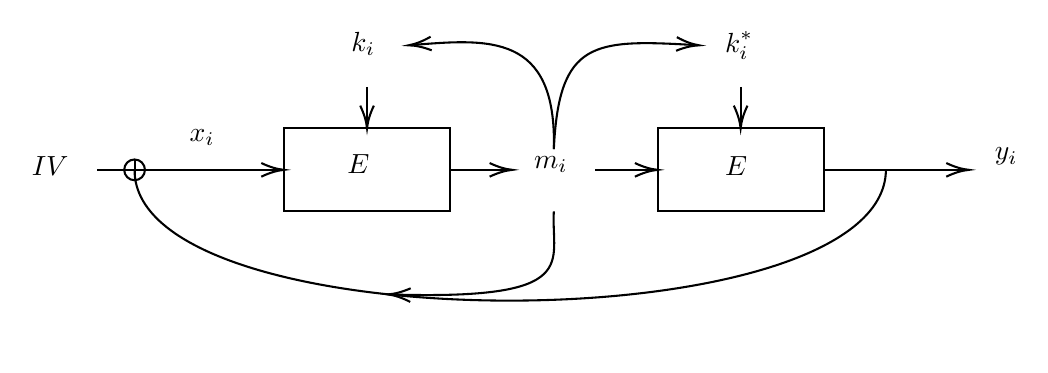
\begin{tikzpicture}[x=0.75pt,y=0.75pt,yscale=-1,xscale=1]
%uncomment if require: \path (0,284); %set diagram left start at 0, and has height of 284

%Shape: Rectangle [id:dp6411361187876574] 
\draw   (140,80) -- (220,80) -- (220,120) -- (140,120) -- cycle ;
%Shape: Rectangle [id:dp60254390298104] 
\draw   (320,80) -- (400,80) -- (400,120) -- (320,120) -- cycle ;
%Straight Lines [id:da8429683136429227] 
\draw    (50,100) -- (138,100) ;
\draw [shift={(140,100)}, rotate = 180] [color={rgb, 255:red, 0; green, 0; blue, 0 }  ][line width=0.75]    (10.93,-3.29) .. controls (6.95,-1.4) and (3.31,-0.3) .. (0,0) .. controls (3.31,0.3) and (6.95,1.4) .. (10.93,3.29)   ;
%Straight Lines [id:da9173601683757953] 
\draw    (220,100) -- (248,100) ;
\draw [shift={(250,100)}, rotate = 180] [color={rgb, 255:red, 0; green, 0; blue, 0 }  ][line width=0.75]    (10.93,-3.29) .. controls (6.95,-1.4) and (3.31,-0.3) .. (0,0) .. controls (3.31,0.3) and (6.95,1.4) .. (10.93,3.29)   ;
%Straight Lines [id:da12298912508957316] 
\draw    (290,100) -- (318,100) ;
\draw [shift={(320,100)}, rotate = 180] [color={rgb, 255:red, 0; green, 0; blue, 0 }  ][line width=0.75]    (10.93,-3.29) .. controls (6.95,-1.4) and (3.31,-0.3) .. (0,0) .. controls (3.31,0.3) and (6.95,1.4) .. (10.93,3.29)   ;
%Flowchart: Or [id:dp9863672822794651] 
\draw   (63,100) .. controls (63,97.24) and (65.24,95) .. (68,95) .. controls (70.76,95) and (73,97.24) .. (73,100) .. controls (73,102.76) and (70.76,105) .. (68,105) .. controls (65.24,105) and (63,102.76) .. (63,100) -- cycle ; \draw   (63,100) -- (73,100) ; \draw   (68,95) -- (68,105) ;
%Straight Lines [id:da23963499757442652] 
\draw    (180,60) -- (180,78) ;
\draw [shift={(180,80)}, rotate = 270] [color={rgb, 255:red, 0; green, 0; blue, 0 }  ][line width=0.75]    (10.93,-3.29) .. controls (6.95,-1.4) and (3.31,-0.3) .. (0,0) .. controls (3.31,0.3) and (6.95,1.4) .. (10.93,3.29)   ;
%Straight Lines [id:da9800234273174513] 
\draw    (360,60) -- (360,78) ;
\draw [shift={(360,80)}, rotate = 270] [color={rgb, 255:red, 0; green, 0; blue, 0 }  ][line width=0.75]    (10.93,-3.29) .. controls (6.95,-1.4) and (3.31,-0.3) .. (0,0) .. controls (3.31,0.3) and (6.95,1.4) .. (10.93,3.29)   ;
%Straight Lines [id:da7622990492580304] 
\draw    (400,100) -- (468,100) ;
\draw [shift={(470,100)}, rotate = 180] [color={rgb, 255:red, 0; green, 0; blue, 0 }  ][line width=0.75]    (10.93,-3.29) .. controls (6.95,-1.4) and (3.31,-0.3) .. (0,0) .. controls (3.31,0.3) and (6.95,1.4) .. (10.93,3.29)   ;
%Curve Lines [id:da3925216319768734] 
\draw    (68,100) .. controls (67.5,184) and (429.5,184) .. (430,100) ;
%Curve Lines [id:da5784855574689107] 
\draw    (270,120) .. controls (268.51,144.88) and (284.34,162.82) .. (191.41,160.04) ;
\draw [shift={(190,160)}, rotate = 361.82] [color={rgb, 255:red, 0; green, 0; blue, 0 }  ][line width=0.75]    (10.93,-3.29) .. controls (6.95,-1.4) and (3.31,-0.3) .. (0,0) .. controls (3.31,0.3) and (6.95,1.4) .. (10.93,3.29)   ;
%Curve Lines [id:da8721444883639864] 
\draw    (270,90) .. controls (271.48,33.85) and (238.51,36.89) .. (201.69,39.86) ;
\draw [shift={(200,40)}, rotate = 355.43] [color={rgb, 255:red, 0; green, 0; blue, 0 }  ][line width=0.75]    (10.93,-3.29) .. controls (6.95,-1.4) and (3.31,-0.3) .. (0,0) .. controls (3.31,0.3) and (6.95,1.4) .. (10.93,3.29)   ;
%Curve Lines [id:da8791512286362857] 
\draw    (270,90) .. controls (272.48,37.53) and (289.16,37.01) .. (338.5,39.91) ;
\draw [shift={(340,40)}, rotate = 183.4] [color={rgb, 255:red, 0; green, 0; blue, 0 }  ][line width=0.75]    (10.93,-3.29) .. controls (6.95,-1.4) and (3.31,-0.3) .. (0,0) .. controls (3.31,0.3) and (6.95,1.4) .. (10.93,3.29)   ;

% Text Node
\draw (17,92) node [anchor=north west][inner sep=0.75pt]   [align=left] {$\displaystyle IV$};
% Text Node
\draw (169,91) node [anchor=north west][inner sep=0.75pt]   [align=left] {$\displaystyle E$};
% Text Node
\draw (351,92) node [anchor=north west][inner sep=0.75pt]   [align=left] {$\displaystyle E$};
% Text Node
\draw (259,92) node [anchor=north west][inner sep=0.75pt]   [align=left] {$\displaystyle m_{i}$};
% Text Node
\draw (93,79) node [anchor=north west][inner sep=0.75pt]   [align=left] {$\displaystyle x_{i}$};
% Text Node
\draw (171,32) node [anchor=north west][inner sep=0.75pt]   [align=left] {$\displaystyle k_{i}$};
% Text Node
\draw (351,32) node [anchor=north west][inner sep=0.75pt]   [align=left] {$\displaystyle k_{i}^{*}$};
% Text Node
\draw (481,88) node [anchor=north west][inner sep=0.75pt]   [align=left] {$\displaystyle y_{i}$};
\end{tikzpicture}
\caption{A block-cipher based CSPRNG}
\label{fig:PetitCSPRNG}
\end{figure}

The formal proof of security is somewhat long and beyond the scope of this paper, but the general idea is that since $m$ is used to update $k^*$, we would need $m$ to reverse-engineer the second block cipher. The security comes from the fact that $m$ is essentially random noise generated by $E$, so a successful hack would be very improbable in polynomial time.

The astute reader will notice that the security of block-cipher based CSPRNGs relies on the security of the underlying block cipher. Indeed, Petit et al.'s construction maintains the security guarantee if and only if the block cipher used actually has the nice cryptographic properties we assume. It is still an open question whether truly crpytographically secure block ciphers exist, though we have some standard block cipher protocols (AES, Blowfish, etc.) that are generally accepted to be secure enough for all purposes. In fact, the NIST standard for block-cipher based CSPRNGs recommends using AES as a reliable block cipher \cite{NIST}.

\subsection{Crpytographically Secure Hash Functions}
We take a small detour to talk about the theory of secure hash functions. We will show that truly cryptographically secure block ciphers exist if and only if truly cryptographically secure hash functions exist. We recall the informal definition of a hash function, namely that it uniformly maps a universe of input to some smaller set of hashes. This idea of uniformity is slightly fuzzy and we will formalize this notion in this section.

\begin{definition}[Hash functions]
A \textit{hash function} is a function $h : U \to [m]$, where $U$ is the universe to be hashed, and $[m] = \{0, 1, \dots, m-1\}$. A \textit{family of hash functions} $\mathcal{H}$ is a subset of all such functions $h$.
\end{definition}

Conventionally we assume $m << |U|$ so we are compressing a large universe of possible inputs into a very small set of hashed values. We notice that this definition is very similar to the definition of a family of random functions, and very different from the lay-conception of a hash function. Rather than talk about the sufficiency of any particular function, it is theoretically more sound to talk about the sufficiency for a family of functions. We introduce one such sufficiency criterion here.

\begin{definition}[$k$-wise independence]\label{def:independent}
A family of hash functions $\mathcal{H}$ is \textit{independent} if for all $x \in U$, $i \in [m]$
$$\underset{h \in \mathcal{H}}{Pr}(h(x) = i) = \frac{1}{m}$$
A family of hash functions $\mathcal{H}$ is \textit{k-independent} if for all distinct combinations $x_1,\dots, x_k \in U$, $i_1, \dots, i_k \in [m]$
$$\underset{h \in \mathcal{H}}{Pr}(\bigwedge^k h(x_j) = i_j) = \frac{1}{m^k}$$
\end{definition}

Independence is sometimes called uniformity. Intuitively, an independent hash function achieves our informal definition, that hashes should be distributed essentially randomly. Given a random function from an independent family, one cannot predict the outcome of any singular hashing with more than random probability. $k$-independence is an even stronger condition. Given even $k$ chances to hash random things, we cannot determine whether we have chosen a function from random or a function from the independent family with more than random probability.

2-independence is theoretically enough for cryptographic applications. One of the main requirements for crpyographic hash functions is that they are \textit{collision-resistant}, meaning it's difficult for a given $h(m)$ to find another $m'$ such that $h(m) = h(m')$ \cite{PractCrypt}. Independence guarantees the probability of finding such $m'$ is $\frac{1}{m}$, as good as we can possibly get. Another requirement is the so-called \textit{avalance effect}, where a small change in the input $m$ drastically changes the hashed value \cite{PractCrypt}. It is clear from Defintion~\ref{def:independent} we have shown that this is a flowery way of defining 2-independence. Finally, a cryptographic hash function should be infeasible to reverse. This is not explicitly satisfied by independence, but is a consequence of $U >> |m|$, since we will have no better way of finding an inverse than by looking through the universe of all possible inputs until we find a match.

In practice, it is difficult to come up with deterministic functions that behave as is they come from a 2-independent family. It is even more difficult to come up with a deterministic function that mimics 2-independence while being hard to reverse. Many of the hash functions commonly used in cryptographic applications (SHA-2, MD5) are functions that are widely believed to be good approximations of cryptographically secure hash functions. But there is no sound mathematical proof that these functions are in fact secure. In the case of MD5, it was revealed that it is not as collision-resistant as originally hoped, and researchers were able to break the encryption in 2004 \cite{MD5}.

There are examples of cryptographic hash functions that are \say{more} provably secure, such as those based on the discrete logarithm or other hard mathematical problems. However, since it is unknown whether these are actually super-polynomial problems, we cannot concretely prove the security of these hash functions. Indeed, as long as $P \overset{?}{=} NP$ is an open problem, we cannot be sure of any of these hash functions \cite{Textbook}.

To finish our survey of cryptographic hashing, we establish the connection between hashing and block ciphers. Recall that a block cipher is, at its core, a function $f(k,x) = y$, where $k,x,y \in \mathbb{F}_2^n$ are binary strings. In other words, we can model $f$ as a function $\mathbb{F}_2^n \times \mathbb{F}_2^n \to \mathbb{F}_2^n$ or, if we concatenate the bits of $k$ and $x$, a function $\mathbb{F}_2^{2n} \to \mathbb{F}_2^n$. We can consider $f$ thus to be a function chosen from the set of functions $h : \mathbb{F}_2^{2n} \to [2^{n+1}]$. The criteria for a secure block cipher (indistinguishability, non-locality) are satisfied by secure hash functions. Non-locality is another way of specifying the avalance effect, and indistinguishability is a consequence of irreversibility. Thus, a secure block cipher exists only if a secure hash function exists. Similarly, since the criteria for secure block ciphers and secure hash functions are essentially one-to-one, a secure hash function exists only if a secure block cipher exists. The two concepts are closely related both in theory and in practice.

\subsection{Hash-based CSPRNG}
We finish this section by describing a CSPRNG based on a cryptographically secure hash function $h$. Suppose $h$ is a secure hash function that returns $2k$ bits. Initialize an internal state $s$ with a random seed. Hash this seed and replace $s := h(s)$. When asked to generate a random number, return the top $k$ bits of $h(s)$ and update $s := h(s)$.

Because of irreversibility, this PRNG resists state-compromise attacks. Because of irreversibility and independence, this PRNG passes the next-bit test. So indeed this is a CSPRNG.

\section{Applications of PRNGs}
Random number generators are very useful in many applications. The most salient and easy to understand is in statistical simulations. We can use random number generators to easily model uncertainty and random sampling. For instance, we may model a uniform distribution with a basic (uniformly-distributed) PRNG. In fact, we may model selection from any distribution by first randomly (uniformly) selecting a value $v \in (0,1)$ and calculating the inverse CDF of $v$ to get the random value. This is very useful for continuous distributions and we may easily modify this method for discrete distributions by giving ranges in which $v$ maps to the different values of the random variable.

In practice, this form of randomness is incredibly useful for simulating games of chance. For instance, dice rolls, poker draws, and roulette spins are all determined with random sampling via random number generation. Outside of the casino but still in the same realm, randomness is required for simulations of random behavior. Both Montecarlo and Las Vegas processes require much of the same random sampling as actual casino simulations and thus use PRNGs in very similar ways \cite{MTWiki}.

\subsection{Randomized Algorithms}
Randomization is also important for a category of algorithms aptly named \textit{randomized algorithms}. Oftentimes deterministic algorithms have not-so-stellar theoretical bounds that may be improved by introducing an element of randomness. In many of these cases, the worst case bound does not improve, but the expected (or average) case improves greatly. We give an example of such an algorithm here [taken from my notes and homework for Prof. Farach-Colton's algorithms seminar, Fall 2020]:
\begin{myindentpar}{1em}
Suppose we are given a string of $2n$ bits in which half of them are \verb|0| and half of them are \verb|1|. Our task is to output the index of a \verb|1|. As an example, if we were given the string \verb|001011|, correct answers would be 2,4, and 5.
\end{myindentpar}
A deterministic algorithm can do no better than to check every bit until we see a \verb|1|, yielding a time complexity of $\mathcal{O}(n)$. However, we can produce a randomized algorithm which randomly checks bits until we find a \verb|1|. Since at each step there is a $\frac{1}{2}$ chance of picking a \verb|1|, by Markov we expect this algorithm to run in $2$ steps, in other words, $\theta(1)$. This is a massive improvement in the average case and justifies our use of randomization. Note that the worst case is arbitrarily bad. We may get extrememly unlucky and always pick the same index to check every time into perpetuity, but the probability of this is vanishingly small. In fact, even a rough analysis with Chebyshev's inequality tells us that we need only check $\mathcal{O}(\sqrt{n})$ indices with high probability. The details are not terribly relevant, but we include them here for completeness:
\begin{myindentpar}{1em}
We treat this random sampling the same as we would flipping a fair coin. Let $X$ be the number of samplings until we get a desired result. This is a geometric RV with $\mu = 2$ and $\sigma^2 = 2$. By Chebyshev,
$$Pr(|X - \mu| \geqslant k\sigma ) \leqslant \frac{1}{k^2}$$
Substituting $k = \sqrt{n}$ we get
$$Pr(X \geqslant 2 + \sqrt{2n}) \leqslant \frac{1}{n}$$
which indeed is the high-probability bound we desire.
\end{myindentpar}

\subsection{Cryptography}
Random bits are necessary for secure communication and data secrecy. In this section, we discuss their applications in generating secure communication channels, maintaining these channels, and ensuring the data passed along these channels is secure.

Random numbers play a large role in many cryptographic schemes. As we've seen in class, random numbers are necessary for Diffie-Hellman type key generation schemes. The secret exponents $k_A$ and $k_B$ are necessarily chosen at random to prevent compromising the security of the cryptosystem. Similarly, in RSA the large primes $p$ and $q$ should be chosen at random (so long as they are not susceptible to attack). For the RSA-based DSA, the value of $d$ (the so-called \textit{nonce}) generated for verification should be done at random \cite{Textbook}. In fact, all non-public values should be generated randomly or pseudorandomly. For the latter, we must use CSPRNGs to be safe from adversarial attacks.

Wherever cryptography is required, random numbers are most likely also required. One notable example is the (now-deprecated) Secure Sockets Layer (SSL) and its successor Transport Layer Security (TLS). TLS is a network standard that aims to authenticate and secure traffic across the Internet. It's designed to prevent man-in-the-middle attacks in addition to providing security from eavesdroppers \cite{TLS}. The specifics of TLS is complex and not all parts are instructive to our discussion, so we will omit the finer details. At a high level, the two ends of the connection initiate a \say{handshake} in which a digital signature is verified. After this, a random, unique session key is generated and shared between the two parties. This key sharing is often done using Diffie-Hellman and requires the generated key to be securely random. TLS is designed so that even if one of the parties' private keys are exposed, any communications in progress would still not be decryptable due to this random session key. In this way, random number generation acts as a security mechanism to protect network traffic \cite{TLS}.

Finally, random numbers are important for storage of passwords and other secrets. Suppose you were in charge of operating IT for a major bank. How would you verify credit card details for your customers? One method you might think to do is just to store a database of credit card numbers and account numbers. But as we've seen in countless cases, storing sensitive information in plaintext is a recipe for massive data breaches and chronic security issues. One potential solution is to hash the plaintext according to a known hash function and only store the hashed value. Then a data breach would not immediately lead to public knowledge of the plaintext data. But this has some potential downsides as well. Imagine a massive data breach where many hashed passwords are revealed. People are unfortunately very predictable, and many of your customers will have used the same password to log into their account. In fact, people are so predictable that there are databases of the most frequently used passwords in a number of different countries, in other words, a frequency analysis of passwords. Then since hash functions are deterministic, one password will hash to the same encrypted value every time a customer uses it. Uh oh! We've created a giant substitution cipher where decryption compromises the bank details of thousands of people. The solution to this problem is to \textit{salt and hash} the plaintext. Generate a unique bit string \textit{salt} concatenate with the plaintext and hash. Instead of storing just the hashed value, also store the salt. This addresses the multiple password problem by forcing the input to the hash function to be unique and thus the outputs to look like random noise \cite{Salt}. Note that storing the salt also doesn't compromise security, since a secure hash function guarantees non-locality so the only way to reverse the hash (even with the salt) is to bruteforce try every possible input. The most common method of generating salts is by generating random numbers with a CSPRNG. Although we aren't guaranteed uniqueness with a PRNG, we're guaranteed that the probability of generating the same number twice to be exceedingly low. In most practical applications, including banking, this is good enough.

\section{RNGs In Practice}
We finish our discussion of PRNGs with an overview of PRNG implementations in common software libraries.

Java's \verb|Random| class is implemented using a Linear Congruential Generator \cite{LCGWiki}. It has recurrence function
$$X_{i+1} = (25214903917X_i + 11) \!\!\!\mod 2^{48}$$
To combat the problem with low-order bits using a power-of-2 modulus, the generator discards the lower 16 bits, only returning the top 32 bits.

The C \verb|rand()| function has a number of implementations, but they are all Linear Congruential Generators \cite{LCGWiki}. The most common implementations (ANSI C, GCC) use recurrence function
$$X_{i+1} = (1103515245X_i + 12345) \!\!\!\mod 2^{31}$$

In C++, \verb|rand()| is still supported but many compilers will warn that it provides limited randomness. In C++ 11, the \verb|<random>| library has implementations of an LCG, MT19937, and a \textit{subtract-and-carry} generator. MT19937 we've discussed as the standard Mersenne Twister implementation. Subtract-and-carry is an implementation of a newer non-linear generator. See the C++ 11 documentation for more details on this.

Most other modern languages and computational software provide implementations of MT19937. The following is an inexhaustive list:\\
Python, Ruby, MATLAB, Maple, PHP, Lisp, Microsoft Excel, SAS, R \cite{MTWiki}.

\bibliography{final}

\end{document}

% List of tex snippets:
%   - tex-header (this)
%   - R      --> \mathbb{R}
%   - Z      --> \mathbb{Z}
%   - B      --> \mathcal{B}
%   - E      --> \mathcal{E}
%   - M      --> \mathcal{M}
%   - m      --> \mathfrak{m}({#1})
%   - normlp --> \norm{{#1}}_{L^{{#2}}}
